\documentclass{standalone}
\usepackage{tikz}
\usetikzlibrary{patterns}
\usetikzlibrary{positioning}
\usetikzlibrary{patterns, positioning}
\usetikzlibrary{shapes.misc}
\usepackage[outline]{contour}
\contourlength{1.5pt} 
\usetikzlibrary{calc}
        \usepackage{relsize}
        \tikzset{fontscale/.style = {font=\relsize{#1}}}

\begin{document}
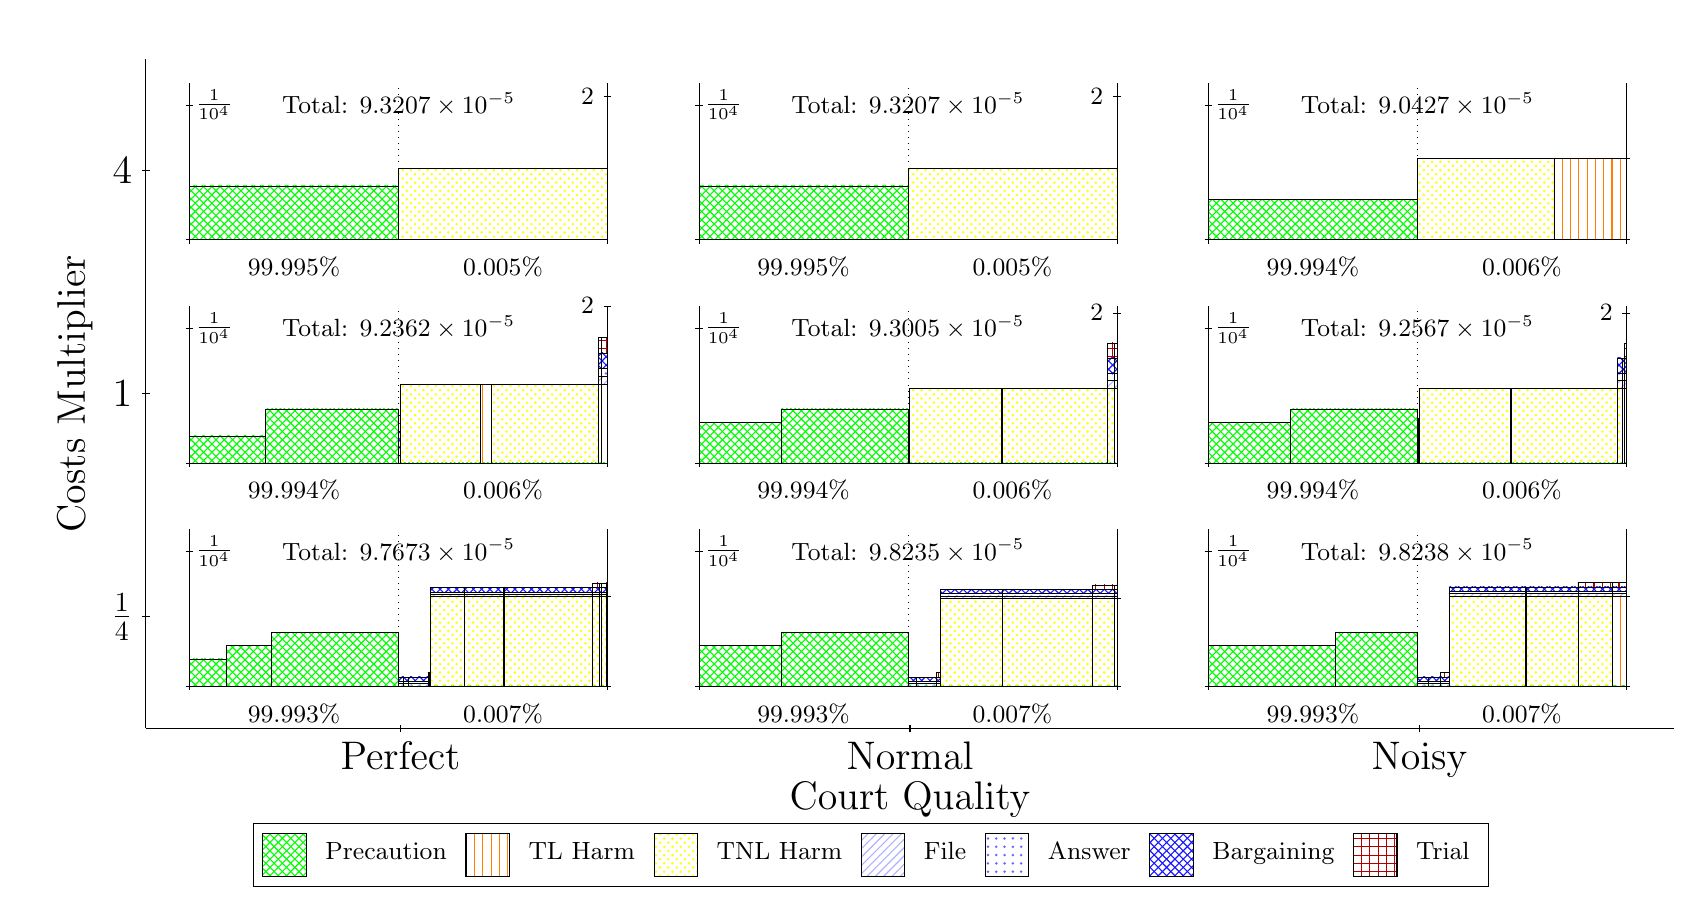
\begin{tikzpicture}
\clip(-0.5,-1.1) rectangle +(20.91,11);
\draw[black] (1,1) -- (1,9.5);
\node[rotate=90, fontscale=2, anchor=center] at (0.1, 5.25) {Costs Multiplier};
\draw[black] (0.95,2.4167) -- (1.05,2.4167);
\node[fontscale=2, anchor=east] at (0.95, 2.4167) {$\frac{1}{4}$};
\draw[black] (0.95,5.25) -- (1.05,5.25);
\node[fontscale=2, anchor=east] at (0.95, 5.25) {1};
\draw[black] (0.95,8.0833) -- (1.05,8.0833);
\node[fontscale=2, anchor=east] at (0.95, 8.0833) {4};

\draw[black] (1,1) -- (20.41,1);
\node[fontscale=2, anchor=center] at (10.705, 0.1) {Court Quality};
\draw[black] (4.235,0.95) -- (4.235,1.05);
\node[fontscale=2, anchor=north] at (4.235, 0.95) {Perfect};
\draw[black] (10.705,0.95) -- (10.705,1.05);
\node[fontscale=2, anchor=north] at (10.705, 0.95) {Normal};
\draw[black] (17.175,0.95) -- (17.175,1.05);
\node[fontscale=2, anchor=north] at (17.175, 0.95) {Noisy};


\draw[pattern=crosshatch, pattern color=green,draw=black,very thin] (1.5556,1.54) rectangle (2.0233,1.8823);
\draw[pattern=crosshatch, pattern color=green,draw=black,very thin] (2.0233,1.54) rectangle (2.5958,2.0534);
\draw[pattern=crosshatch, pattern color=green,draw=black,very thin] (2.5958,1.54) rectangle (4.21,2.2246);
\draw[pattern=crosshatch, pattern color=green,draw=black,very thin] (4.21,1.54) rectangle (4.2654,1.54);
\draw[pattern=north east lines, pattern color=blue!30,draw=black,very thin] (4.21,1.54) rectangle (4.2654,1.5685);
\draw[pattern=dots,  pattern color=blue!60,draw=black,very thin] (4.21,1.5685) rectangle (4.2654,1.5969);
\draw[pattern=crosshatch,      pattern color=blue!90,draw=black,very thin] (4.21,1.5969) rectangle (4.2654,1.6537);
\draw[pattern=crosshatch, pattern color=green,draw=black,very thin] (4.2654,1.54) rectangle (4.3388,1.54);
\draw[pattern=north east lines, pattern color=blue!30,draw=black,very thin] (4.2654,1.54) rectangle (4.3388,1.5685);
\draw[pattern=dots,  pattern color=blue!60,draw=black,very thin] (4.2654,1.5685) rectangle (4.3388,1.5969);
\draw[pattern=crosshatch,      pattern color=blue!90,draw=black,very thin] (4.2654,1.5969) rectangle (4.3388,1.6537);
\draw[pattern=crosshatch, pattern color=green,draw=black,very thin] (4.3388,1.54) rectangle (4.5818,1.54);
\draw[pattern=north east lines, pattern color=blue!30,draw=black,very thin] (4.3388,1.54) rectangle (4.5818,1.5685);
\draw[pattern=dots,  pattern color=blue!60,draw=black,very thin] (4.3388,1.5685) rectangle (4.5818,1.5969);
\draw[pattern=crosshatch,      pattern color=blue!90,draw=black,very thin] (4.3388,1.5969) rectangle (4.5818,1.6538);
\draw[pattern=crosshatch, pattern color=green,draw=black,very thin] (4.5818,1.54) rectangle (4.5968,1.54);
\draw[pattern=north east lines, pattern color=blue!30,draw=black,very thin] (4.5818,1.54) rectangle (4.5968,1.5685);
\draw[pattern=dots,  pattern color=blue!60,draw=black,very thin] (4.5818,1.5685) rectangle (4.5968,1.5969);
\draw[pattern=crosshatch,      pattern color=blue!90,draw=black,very thin] (4.5818,1.5969) rectangle (4.5968,1.6537);
\draw[pattern=grid,            pattern color=red!70!black,draw=black,very thin] (4.5818,1.6537) rectangle (4.5968,1.7106);
\draw[pattern=crosshatch, pattern color=green,draw=black,very thin] (4.5968,1.54) rectangle (4.6095,1.54);
\draw[pattern=north east lines, pattern color=blue!30,draw=black,very thin] (4.5968,1.54) rectangle (4.6095,1.5685);
\draw[pattern=dots,  pattern color=blue!60,draw=black,very thin] (4.5968,1.5685) rectangle (4.6095,1.5969);
\draw[pattern=crosshatch,      pattern color=blue!90,draw=black,very thin] (4.5968,1.5969) rectangle (4.6095,1.6537);
\draw[pattern=grid,            pattern color=red!70!black,draw=black,very thin] (4.5968,1.6537) rectangle (4.6095,1.7106);
\draw[pattern=crosshatch, pattern color=green,draw=black,very thin] (4.6095,1.54) rectangle (5.0391,1.54);
\draw[pattern=crosshatch dots, pattern color=yellow,draw=black,very thin] (4.6095,1.54) rectangle (5.0391,2.6772);
\draw[pattern=north east lines, pattern color=blue!30,draw=black,very thin] (4.6095,2.6772) rectangle (5.0391,2.7056);
\draw[pattern=dots,  pattern color=blue!60,draw=black,very thin] (4.6095,2.7056) rectangle (5.0391,2.734);
\draw[pattern=crosshatch,      pattern color=blue!90,draw=black,very thin] (4.6095,2.734) rectangle (5.0391,2.7909);
\draw[pattern=crosshatch, pattern color=green,draw=black,very thin] (5.0391,1.54) rectangle (5.0501,1.54);
\draw[pattern=vertical lines, pattern color=orange,draw=black,very thin] (5.0391,1.54) rectangle (5.0501,2.6772);
\draw[pattern=north east lines, pattern color=blue!30,draw=black,very thin] (5.0391,2.6772) rectangle (5.0501,2.7056);
\draw[pattern=dots,  pattern color=blue!60,draw=black,very thin] (5.0391,2.7056) rectangle (5.0501,2.734);
\draw[pattern=crosshatch,      pattern color=blue!90,draw=black,very thin] (5.0391,2.734) rectangle (5.0501,2.7909);
\draw[pattern=crosshatch, pattern color=green,draw=black,very thin] (5.0501,1.54) rectangle (5.5449,1.54);
\draw[pattern=crosshatch dots, pattern color=yellow,draw=black,very thin] (5.0501,1.54) rectangle (5.5449,2.6772);
\draw[pattern=north east lines, pattern color=blue!30,draw=black,very thin] (5.0501,2.6772) rectangle (5.5449,2.7056);
\draw[pattern=dots,  pattern color=blue!60,draw=black,very thin] (5.0501,2.7056) rectangle (5.5449,2.734);
\draw[pattern=crosshatch,      pattern color=blue!90,draw=black,very thin] (5.0501,2.734) rectangle (5.5449,2.7909);
\draw[pattern=crosshatch, pattern color=green,draw=black,very thin] (5.5449,1.54) rectangle (5.5546,1.54);
\draw[pattern=vertical lines, pattern color=orange,draw=black,very thin] (5.5449,1.54) rectangle (5.5546,2.6772);
\draw[pattern=north east lines, pattern color=blue!30,draw=black,very thin] (5.5449,2.6772) rectangle (5.5546,2.7056);
\draw[pattern=dots,  pattern color=blue!60,draw=black,very thin] (5.5449,2.7056) rectangle (5.5546,2.734);
\draw[pattern=crosshatch,      pattern color=blue!90,draw=black,very thin] (5.5449,2.734) rectangle (5.5546,2.7909);
\draw[pattern=crosshatch, pattern color=green,draw=black,very thin] (5.5546,1.54) rectangle (6.6757,1.54);
\draw[pattern=crosshatch dots, pattern color=yellow,draw=black,very thin] (5.5546,1.54) rectangle (6.6757,2.6772);
\draw[pattern=north east lines, pattern color=blue!30,draw=black,very thin] (5.5546,2.6772) rectangle (6.6757,2.7056);
\draw[pattern=dots,  pattern color=blue!60,draw=black,very thin] (5.5546,2.7056) rectangle (6.6757,2.734);
\draw[pattern=crosshatch,      pattern color=blue!90,draw=black,very thin] (5.5546,2.734) rectangle (6.6757,2.7909);
\draw[pattern=crosshatch, pattern color=green,draw=black,very thin] (6.6757,1.54) rectangle (6.762,1.54);
\draw[pattern=crosshatch dots, pattern color=yellow,draw=black,very thin] (6.6757,1.54) rectangle (6.762,2.6772);
\draw[pattern=north east lines, pattern color=blue!30,draw=black,very thin] (6.6757,2.6772) rectangle (6.762,2.7056);
\draw[pattern=dots,  pattern color=blue!60,draw=black,very thin] (6.6757,2.7056) rectangle (6.762,2.734);
\draw[pattern=crosshatch,      pattern color=blue!90,draw=black,very thin] (6.6757,2.734) rectangle (6.762,2.7909);
\draw[pattern=grid,            pattern color=red!70!black,draw=black,very thin] (6.6757,2.7909) rectangle (6.762,2.8477);
\draw[pattern=crosshatch, pattern color=green,draw=black,very thin] (6.762,1.54) rectangle (6.7894,1.54);
\draw[pattern=vertical lines, pattern color=orange,draw=black,very thin] (6.762,1.54) rectangle (6.7894,2.6772);
\draw[pattern=north east lines, pattern color=blue!30,draw=black,very thin] (6.762,2.6772) rectangle (6.7894,2.7056);
\draw[pattern=dots,  pattern color=blue!60,draw=black,very thin] (6.762,2.7056) rectangle (6.7894,2.734);
\draw[pattern=crosshatch,      pattern color=blue!90,draw=black,very thin] (6.762,2.734) rectangle (6.7894,2.7909);
\draw[pattern=grid,            pattern color=red!70!black,draw=black,very thin] (6.762,2.7909) rectangle (6.7894,2.8477);
\draw[pattern=crosshatch, pattern color=green,draw=black,very thin] (6.7894,1.54) rectangle (6.8427,1.54);
\draw[pattern=crosshatch dots, pattern color=yellow,draw=black,very thin] (6.7894,1.54) rectangle (6.8427,2.6772);
\draw[pattern=north east lines, pattern color=blue!30,draw=black,very thin] (6.7894,2.6772) rectangle (6.8427,2.7056);
\draw[pattern=dots,  pattern color=blue!60,draw=black,very thin] (6.7894,2.7056) rectangle (6.8427,2.734);
\draw[pattern=crosshatch,      pattern color=blue!90,draw=black,very thin] (6.7894,2.734) rectangle (6.8427,2.7909);
\draw[pattern=grid,            pattern color=red!70!black,draw=black,very thin] (6.7894,2.7909) rectangle (6.8427,2.8477);
\draw[pattern=crosshatch, pattern color=green,draw=black,very thin] (6.8427,1.54) rectangle (6.8644,1.54);
\draw[pattern=vertical lines, pattern color=orange,draw=black,very thin] (6.8427,1.54) rectangle (6.8644,2.6772);
\draw[pattern=north east lines, pattern color=blue!30,draw=black,very thin] (6.8427,2.6772) rectangle (6.8644,2.7056);
\draw[pattern=dots,  pattern color=blue!60,draw=black,very thin] (6.8427,2.7056) rectangle (6.8644,2.734);
\draw[pattern=crosshatch,      pattern color=blue!90,draw=black,very thin] (6.8427,2.734) rectangle (6.8644,2.7909);
\draw[pattern=grid,            pattern color=red!70!black,draw=black,very thin] (6.8427,2.7909) rectangle (6.8644,2.8477);
\node[font=\small,text=black,anchor=north] at (4.21, 3.5333) {Total: $9.7673\times 10^{-5}$};
\draw[black,very thin] (1.5556,1.54) -- (1.5556,3.5333);
\draw[black,very thin] (1.5056,1.54) -- (1.6056,1.54);
\node[font=\small,text=black, anchor=west] at (1.5056, 1.54) {};
\draw[black,very thin] (1.5056,3.2515) -- (1.6056,3.2515);
\node[font=\small,text=black, anchor=west] at (1.5056, 3.2515) {$\frac{1}{10^{4}}$};

\draw[black,dotted,very thin] (4.21,1.5998) -- (4.21,3.4735);
\draw[black,very thin] (6.8644,1.54) -- (6.8644,3.5333);
\draw[black,very thin] (6.8144,1.54) -- (6.9144,1.54);
\node[font=\small,text=black, anchor=east] at (6.8144, 1.54) {\contour{white}{}};
\draw[black,very thin] (6.8144,2.6771) -- (6.9144,2.6771);
\node[font=\small,text=black, anchor=east] at (6.8144, 2.6771) {\contour{white}{}};

\draw[black,very thin] (1.5556,1.54) -- (6.8644,1.54);
\draw[black,very thin] (1.5556,1.49) -- (1.5556,1.59);
\node[font=\small,text=black, anchor=north] at (1.5556, 1.49) {};
\draw[black,very thin] (6.8644,1.49) -- (6.8644,1.59);
\node[font=\small,text=black, anchor=north] at (6.8644, 1.49) {};

\node[font=\small,text=black,anchor=south] at (2.8828, 0.94) {99.993\%};
\node[font=\small,text=black,anchor=south] at (5.5372, 0.94) {0.007\%};

\draw[pattern=crosshatch, pattern color=green,draw=black,very thin] (8.0256,1.54) rectangle (9.0658,2.0534);
\draw[pattern=crosshatch, pattern color=green,draw=black,very thin] (9.0658,1.54) rectangle (10.68,2.2246);
\draw[pattern=crosshatch, pattern color=green,draw=black,very thin] (10.68,1.54) rectangle (10.791,1.54);
\draw[pattern=north east lines, pattern color=blue!30,draw=black,very thin] (10.68,1.54) rectangle (10.791,1.5679);
\draw[pattern=dots,  pattern color=blue!60,draw=black,very thin] (10.68,1.5679) rectangle (10.791,1.5958);
\draw[pattern=crosshatch,      pattern color=blue!90,draw=black,very thin] (10.68,1.5958) rectangle (10.791,1.6516);
\draw[pattern=crosshatch, pattern color=green,draw=black,very thin] (10.791,1.54) rectangle (11.039,1.54);
\draw[pattern=north east lines, pattern color=blue!30,draw=black,very thin] (10.791,1.54) rectangle (11.039,1.5679);
\draw[pattern=dots,  pattern color=blue!60,draw=black,very thin] (10.791,1.5679) rectangle (11.039,1.5958);
\draw[pattern=crosshatch,      pattern color=blue!90,draw=black,very thin] (10.791,1.5958) rectangle (11.039,1.6516);
\draw[pattern=crosshatch, pattern color=green,draw=black,very thin] (11.039,1.54) rectangle (11.087,1.54);
\draw[pattern=north east lines, pattern color=blue!30,draw=black,very thin] (11.039,1.54) rectangle (11.087,1.5679);
\draw[pattern=dots,  pattern color=blue!60,draw=black,very thin] (11.039,1.5679) rectangle (11.087,1.5958);
\draw[pattern=crosshatch,      pattern color=blue!90,draw=black,very thin] (11.039,1.5958) rectangle (11.087,1.6516);
\draw[pattern=grid,            pattern color=red!70!black,draw=black,very thin] (11.039,1.6516) rectangle (11.087,1.7074);
\draw[pattern=crosshatch, pattern color=green,draw=black,very thin] (11.087,1.54) rectangle (11.879,1.54);
\draw[pattern=crosshatch dots, pattern color=yellow,draw=black,very thin] (11.087,1.54) rectangle (11.879,2.6558);
\draw[pattern=north east lines, pattern color=blue!30,draw=black,very thin] (11.087,2.6558) rectangle (11.879,2.6837);
\draw[pattern=dots,  pattern color=blue!60,draw=black,very thin] (11.087,2.6837) rectangle (11.879,2.7116);
\draw[pattern=crosshatch,      pattern color=blue!90,draw=black,very thin] (11.087,2.7116) rectangle (11.879,2.7674);
\draw[pattern=crosshatch, pattern color=green,draw=black,very thin] (11.879,1.54) rectangle (11.881,1.54);
\draw[pattern=vertical lines, pattern color=orange,draw=black,very thin] (11.879,1.54) rectangle (11.881,2.6558);
\draw[pattern=north east lines, pattern color=blue!30,draw=black,very thin] (11.879,2.6558) rectangle (11.881,2.6837);
\draw[pattern=dots,  pattern color=blue!60,draw=black,very thin] (11.879,2.6837) rectangle (11.881,2.7116);
\draw[pattern=crosshatch,      pattern color=blue!90,draw=black,very thin] (11.879,2.7116) rectangle (11.881,2.7674);
\draw[pattern=crosshatch, pattern color=green,draw=black,very thin] (11.881,1.54) rectangle (13.024,1.54);
\draw[pattern=crosshatch dots, pattern color=yellow,draw=black,very thin] (11.881,1.54) rectangle (13.024,2.6559);
\draw[pattern=north east lines, pattern color=blue!30,draw=black,very thin] (11.881,2.6559) rectangle (13.024,2.6838);
\draw[pattern=dots,  pattern color=blue!60,draw=black,very thin] (11.881,2.6838) rectangle (13.024,2.7116);
\draw[pattern=crosshatch,      pattern color=blue!90,draw=black,very thin] (11.881,2.7116) rectangle (13.024,2.7674);
\draw[pattern=crosshatch, pattern color=green,draw=black,very thin] (13.024,1.54) rectangle (13.3,1.54);
\draw[pattern=crosshatch dots, pattern color=yellow,draw=black,very thin] (13.024,1.54) rectangle (13.3,2.6558);
\draw[pattern=north east lines, pattern color=blue!30,draw=black,very thin] (13.024,2.6558) rectangle (13.3,2.6837);
\draw[pattern=dots,  pattern color=blue!60,draw=black,very thin] (13.024,2.6837) rectangle (13.3,2.7116);
\draw[pattern=crosshatch,      pattern color=blue!90,draw=black,very thin] (13.024,2.7116) rectangle (13.3,2.7674);
\draw[pattern=grid,            pattern color=red!70!black,draw=black,very thin] (13.024,2.7674) rectangle (13.3,2.8232);
\draw[pattern=crosshatch, pattern color=green,draw=black,very thin] (13.3,1.54) rectangle (13.334,1.54);
\draw[pattern=vertical lines, pattern color=orange,draw=black,very thin] (13.3,1.54) rectangle (13.334,2.6558);
\draw[pattern=north east lines, pattern color=blue!30,draw=black,very thin] (13.3,2.6558) rectangle (13.334,2.6837);
\draw[pattern=dots,  pattern color=blue!60,draw=black,very thin] (13.3,2.6837) rectangle (13.334,2.7116);
\draw[pattern=crosshatch,      pattern color=blue!90,draw=black,very thin] (13.3,2.7116) rectangle (13.334,2.7674);
\draw[pattern=grid,            pattern color=red!70!black,draw=black,very thin] (13.3,2.7674) rectangle (13.334,2.8232);
\node[font=\small,text=black,anchor=north] at (10.68, 3.5333) {Total: $9.8235\times 10^{-5}$};
\draw[black,very thin] (8.0256,1.54) -- (8.0256,3.5333);
\draw[black,very thin] (7.9756,1.54) -- (8.0756,1.54);
\node[font=\small,text=black, anchor=west] at (7.9756, 1.54) {};
\draw[black,very thin] (7.9756,3.2515) -- (8.0756,3.2515);
\node[font=\small,text=black, anchor=west] at (7.9756, 3.2515) {$\frac{1}{10^{4}}$};

\draw[black,dotted,very thin] (10.68,1.5998) -- (10.68,3.4735);
\draw[black,very thin] (13.334,1.54) -- (13.334,3.5333);
\draw[black,very thin] (13.284,1.54) -- (13.384,1.54);
\node[font=\small,text=black, anchor=east] at (13.284, 1.54) {\contour{white}{}};
\draw[black,very thin] (13.284,2.6558) -- (13.384,2.6558);
\node[font=\small,text=black, anchor=east] at (13.284, 2.6558) {\contour{white}{}};

\draw[black,very thin] (8.0256,1.54) -- (13.334,1.54);
\draw[black,very thin] (8.0256,1.49) -- (8.0256,1.59);
\node[font=\small,text=black, anchor=north] at (8.0256, 1.49) {};
\draw[black,very thin] (13.334,1.49) -- (13.334,1.59);
\node[font=\small,text=black, anchor=north] at (13.334, 1.49) {};

\node[font=\small,text=black,anchor=south] at (9.3528, 0.94) {99.993\%};
\node[font=\small,text=black,anchor=south] at (12.007, 0.94) {0.007\%};

\draw[pattern=crosshatch, pattern color=green,draw=black,very thin] (14.496,1.54) rectangle (16.11,2.0534);
\draw[pattern=crosshatch, pattern color=green,draw=black,very thin] (16.11,1.54) rectangle (17.15,2.2246);
\draw[pattern=crosshatch, pattern color=green,draw=black,very thin] (17.15,1.54) rectangle (17.29,1.54);
\draw[pattern=north east lines, pattern color=blue!30,draw=black,very thin] (17.15,1.54) rectangle (17.29,1.5686);
\draw[pattern=dots,  pattern color=blue!60,draw=black,very thin] (17.15,1.5686) rectangle (17.29,1.5972);
\draw[pattern=crosshatch,      pattern color=blue!90,draw=black,very thin] (17.15,1.5972) rectangle (17.29,1.6543);
\draw[pattern=crosshatch, pattern color=green,draw=black,very thin] (17.29,1.54) rectangle (17.445,1.54);
\draw[pattern=north east lines, pattern color=blue!30,draw=black,very thin] (17.29,1.54) rectangle (17.445,1.5686);
\draw[pattern=dots,  pattern color=blue!60,draw=black,very thin] (17.29,1.5686) rectangle (17.445,1.5972);
\draw[pattern=crosshatch,      pattern color=blue!90,draw=black,very thin] (17.29,1.5972) rectangle (17.445,1.6543);
\draw[pattern=crosshatch, pattern color=green,draw=black,very thin] (17.445,1.54) rectangle (17.548,1.54);
\draw[pattern=north east lines, pattern color=blue!30,draw=black,very thin] (17.445,1.54) rectangle (17.548,1.5686);
\draw[pattern=dots,  pattern color=blue!60,draw=black,very thin] (17.445,1.5686) rectangle (17.548,1.5972);
\draw[pattern=crosshatch,      pattern color=blue!90,draw=black,very thin] (17.445,1.5972) rectangle (17.548,1.6543);
\draw[pattern=grid,            pattern color=red!70!black,draw=black,very thin] (17.445,1.6543) rectangle (17.548,1.7114);
\draw[pattern=crosshatch, pattern color=green,draw=black,very thin] (17.548,1.54) rectangle (18.516,1.54);
\draw[pattern=crosshatch dots, pattern color=yellow,draw=black,very thin] (17.548,1.54) rectangle (18.516,2.6824);
\draw[pattern=north east lines, pattern color=blue!30,draw=black,very thin] (17.548,2.6824) rectangle (18.516,2.7109);
\draw[pattern=dots,  pattern color=blue!60,draw=black,very thin] (17.548,2.7109) rectangle (18.516,2.7395);
\draw[pattern=crosshatch,      pattern color=blue!90,draw=black,very thin] (17.548,2.7395) rectangle (18.516,2.7966);
\draw[pattern=crosshatch, pattern color=green,draw=black,very thin] (18.516,1.54) rectangle (18.528,1.54);
\draw[pattern=vertical lines, pattern color=orange,draw=black,very thin] (18.516,1.54) rectangle (18.528,2.6824);
\draw[pattern=north east lines, pattern color=blue!30,draw=black,very thin] (18.516,2.6824) rectangle (18.528,2.7109);
\draw[pattern=dots,  pattern color=blue!60,draw=black,very thin] (18.516,2.7109) rectangle (18.528,2.7395);
\draw[pattern=crosshatch,      pattern color=blue!90,draw=black,very thin] (18.516,2.7395) rectangle (18.528,2.7966);
\draw[pattern=crosshatch, pattern color=green,draw=black,very thin] (18.528,1.54) rectangle (19.188,1.54);
\draw[pattern=crosshatch dots, pattern color=yellow,draw=black,very thin] (18.528,1.54) rectangle (19.188,2.6824);
\draw[pattern=north east lines, pattern color=blue!30,draw=black,very thin] (18.528,2.6824) rectangle (19.188,2.7109);
\draw[pattern=dots,  pattern color=blue!60,draw=black,very thin] (18.528,2.7109) rectangle (19.188,2.7395);
\draw[pattern=crosshatch,      pattern color=blue!90,draw=black,very thin] (18.528,2.7395) rectangle (19.188,2.7966);
\draw[pattern=crosshatch, pattern color=green,draw=black,very thin] (19.188,1.54) rectangle (19.621,1.54);
\draw[pattern=crosshatch dots, pattern color=yellow,draw=black,very thin] (19.188,1.54) rectangle (19.621,2.6824);
\draw[pattern=north east lines, pattern color=blue!30,draw=black,very thin] (19.188,2.6824) rectangle (19.621,2.7109);
\draw[pattern=dots,  pattern color=blue!60,draw=black,very thin] (19.188,2.7109) rectangle (19.621,2.7395);
\draw[pattern=crosshatch,      pattern color=blue!90,draw=black,very thin] (19.188,2.7395) rectangle (19.621,2.7966);
\draw[pattern=grid,            pattern color=red!70!black,draw=black,very thin] (19.188,2.7966) rectangle (19.621,2.8537);
\draw[pattern=crosshatch, pattern color=green,draw=black,very thin] (19.621,1.54) rectangle (19.804,1.54);
\draw[pattern=vertical lines, pattern color=orange,draw=black,very thin] (19.621,1.54) rectangle (19.804,2.6824);
\draw[pattern=north east lines, pattern color=blue!30,draw=black,very thin] (19.621,2.6824) rectangle (19.804,2.7109);
\draw[pattern=dots,  pattern color=blue!60,draw=black,very thin] (19.621,2.7109) rectangle (19.804,2.7395);
\draw[pattern=crosshatch,      pattern color=blue!90,draw=black,very thin] (19.621,2.7395) rectangle (19.804,2.7966);
\draw[pattern=grid,            pattern color=red!70!black,draw=black,very thin] (19.621,2.7966) rectangle (19.804,2.8537);
\node[font=\small,text=black,anchor=north] at (17.15, 3.5333) {Total: $9.8238\times 10^{-5}$};
\draw[black,very thin] (14.496,1.54) -- (14.496,3.5333);
\draw[black,very thin] (14.446,1.54) -- (14.546,1.54);
\node[font=\small,text=black, anchor=west] at (14.446, 1.54) {};
\draw[black,very thin] (14.446,3.2515) -- (14.546,3.2515);
\node[font=\small,text=black, anchor=west] at (14.446, 3.2515) {$\frac{1}{10^{4}}$};

\draw[black,dotted,very thin] (17.15,1.5998) -- (17.15,3.4735);
\draw[black,very thin] (19.804,1.54) -- (19.804,3.5333);
\draw[black,very thin] (19.754,1.54) -- (19.854,1.54);
\node[font=\small,text=black, anchor=east] at (19.754, 1.54) {\contour{white}{}};
\draw[black,very thin] (19.754,2.6823) -- (19.854,2.6823);
\node[font=\small,text=black, anchor=east] at (19.754, 2.6823) {\contour{white}{}};

\draw[black,very thin] (14.496,1.54) -- (19.804,1.54);
\draw[black,very thin] (14.496,1.49) -- (14.496,1.59);
\node[font=\small,text=black, anchor=north] at (14.496, 1.49) {};
\draw[black,very thin] (19.804,1.49) -- (19.804,1.59);
\node[font=\small,text=black, anchor=north] at (19.804, 1.49) {};

\node[font=\small,text=black,anchor=south] at (15.823, 0.94) {99.993\%};
\node[font=\small,text=black,anchor=south] at (18.477, 0.94) {0.007\%};

\draw[pattern=crosshatch, pattern color=green,draw=black,very thin] (1.5556,4.3733) rectangle (2.5234,4.7156);
\draw[pattern=crosshatch, pattern color=green,draw=black,very thin] (2.5234,4.3733) rectangle (4.21,5.0579);
\draw[pattern=crosshatch, pattern color=green,draw=black,very thin] (4.21,4.3733) rectangle (4.2269,4.3734);
\draw[pattern=north east lines, pattern color=blue!30,draw=black,very thin] (4.21,4.3734) rectangle (4.2269,4.473);
\draw[pattern=dots,  pattern color=blue!60,draw=black,very thin] (4.21,4.473) rectangle (4.2269,4.5727);
\draw[pattern=crosshatch,      pattern color=blue!90,draw=black,very thin] (4.21,4.5727) rectangle (4.2269,4.772);
\draw[pattern=grid,            pattern color=red!70!black,draw=black,very thin] (4.21,4.772) rectangle (4.2269,4.9713);
\draw[pattern=crosshatch, pattern color=green,draw=black,very thin] (4.2269,4.3733) rectangle (5.2523,4.3734);
\draw[pattern=crosshatch dots, pattern color=yellow,draw=black,very thin] (4.2269,4.3734) rectangle (5.2523,5.37);
\draw[pattern=crosshatch, pattern color=green,draw=black,very thin] (5.2523,4.3733) rectangle (5.3891,4.3734);
\draw[pattern=vertical lines, pattern color=orange,draw=black,very thin] (5.2523,4.3734) rectangle (5.3891,5.37);
\draw[pattern=crosshatch, pattern color=green,draw=black,very thin] (5.3891,4.3733) rectangle (6.7449,4.3734);
\draw[pattern=crosshatch dots, pattern color=yellow,draw=black,very thin] (5.3891,4.3734) rectangle (6.7449,5.37);
\draw[pattern=crosshatch, pattern color=green,draw=black,very thin] (6.7449,4.3733) rectangle (6.7808,4.3734);
\draw[pattern=crosshatch dots, pattern color=yellow,draw=black,very thin] (6.7449,4.3734) rectangle (6.7808,5.37);
\draw[pattern=north east lines, pattern color=blue!30,draw=black,very thin] (6.7449,5.37) rectangle (6.7808,5.4697);
\draw[pattern=dots,  pattern color=blue!60,draw=black,very thin] (6.7449,5.4697) rectangle (6.7808,5.5693);
\draw[pattern=crosshatch,      pattern color=blue!90,draw=black,very thin] (6.7449,5.5693) rectangle (6.7808,5.7687);
\draw[pattern=grid,            pattern color=red!70!black,draw=black,very thin] (6.7449,5.7687) rectangle (6.7808,5.968);
\draw[pattern=crosshatch, pattern color=green,draw=black,very thin] (6.7808,4.3733) rectangle (6.8644,4.3734);
\draw[pattern=vertical lines, pattern color=orange,draw=black,very thin] (6.7808,4.3734) rectangle (6.8644,5.37);
\draw[pattern=north east lines, pattern color=blue!30,draw=black,very thin] (6.7808,5.37) rectangle (6.8644,5.4697);
\draw[pattern=dots,  pattern color=blue!60,draw=black,very thin] (6.7808,5.4697) rectangle (6.8644,5.5693);
\draw[pattern=crosshatch,      pattern color=blue!90,draw=black,very thin] (6.7808,5.5693) rectangle (6.8644,5.7687);
\draw[pattern=grid,            pattern color=red!70!black,draw=black,very thin] (6.7808,5.7687) rectangle (6.8644,5.968);
\node[font=\small,text=black,anchor=north] at (4.21, 6.3667) {Total: $9.2362\times 10^{-5}$};
\draw[black,very thin] (1.5556,4.3733) -- (1.5556,6.3667);
\draw[black,very thin] (1.5056,4.3733) -- (1.6056,4.3733);
\node[font=\small,text=black, anchor=west] at (1.5056, 4.3733) {};
\draw[black,very thin] (1.5056,6.0848) -- (1.6056,6.0848);
\node[font=\small,text=black, anchor=west] at (1.5056, 6.0848) {$\frac{1}{10^{4}}$};

\draw[black,dotted,very thin] (4.21,4.4331) -- (4.21,6.3069);
\draw[black,very thin] (6.8644,4.3733) -- (6.8644,6.3667);
\draw[black,very thin] (6.8144,6.3666) -- (6.9144,6.3666);
\node[font=\small,text=black, anchor=east] at (6.8144, 6.3666) {\contour{white}{2}};

\draw[black,very thin] (1.5556,4.3733) -- (6.8644,4.3733);
\draw[black,very thin] (1.5556,4.3233) -- (1.5556,4.4233);
\node[font=\small,text=black, anchor=north] at (1.5556, 4.3233) {};
\draw[black,very thin] (6.8644,4.3233) -- (6.8644,4.4233);
\node[font=\small,text=black, anchor=north] at (6.8644, 4.3233) {};

\node[font=\small,text=black,anchor=south] at (2.8828, 3.7733) {99.994\%};
\node[font=\small,text=black,anchor=south] at (5.5372, 3.7733) {0.006\%};

\draw[pattern=crosshatch, pattern color=green,draw=black,very thin] (8.0256,4.3733) rectangle (9.0658,4.8868);
\draw[pattern=crosshatch, pattern color=green,draw=black,very thin] (9.0658,4.3733) rectangle (10.68,5.0579);
\draw[pattern=crosshatch, pattern color=green,draw=black,very thin] (10.68,4.3733) rectangle (10.7,4.3734);
\draw[pattern=north east lines, pattern color=blue!30,draw=black,very thin] (10.68,4.3734) rectangle (10.7,4.4685);
\draw[pattern=dots,  pattern color=blue!60,draw=black,very thin] (10.68,4.4685) rectangle (10.7,4.5637);
\draw[pattern=crosshatch,      pattern color=blue!90,draw=black,very thin] (10.68,4.5637) rectangle (10.7,4.754);
\draw[pattern=grid,            pattern color=red!70!black,draw=black,very thin] (10.68,4.754) rectangle (10.7,4.9444);
\draw[pattern=crosshatch, pattern color=green,draw=black,very thin] (10.7,4.3733) rectangle (11.865,4.3734);
\draw[pattern=crosshatch dots, pattern color=yellow,draw=black,very thin] (10.7,4.3734) rectangle (11.865,5.3251);
\draw[pattern=crosshatch, pattern color=green,draw=black,very thin] (11.865,4.3733) rectangle (11.877,4.3734);
\draw[pattern=vertical lines, pattern color=orange,draw=black,very thin] (11.865,4.3734) rectangle (11.877,5.3251);
\draw[pattern=crosshatch, pattern color=green,draw=black,very thin] (11.877,4.3733) rectangle (13.216,4.3734);
\draw[pattern=crosshatch dots, pattern color=yellow,draw=black,very thin] (11.877,4.3734) rectangle (13.216,5.3251);
\draw[pattern=crosshatch, pattern color=green,draw=black,very thin] (13.216,4.3733) rectangle (13.304,4.3734);
\draw[pattern=crosshatch dots, pattern color=yellow,draw=black,very thin] (13.216,4.3734) rectangle (13.304,5.3251);
\draw[pattern=north east lines, pattern color=blue!30,draw=black,very thin] (13.216,5.3251) rectangle (13.304,5.4202);
\draw[pattern=dots,  pattern color=blue!60,draw=black,very thin] (13.216,5.4202) rectangle (13.304,5.5154);
\draw[pattern=crosshatch,      pattern color=blue!90,draw=black,very thin] (13.216,5.5154) rectangle (13.304,5.7058);
\draw[pattern=grid,            pattern color=red!70!black,draw=black,very thin] (13.216,5.7058) rectangle (13.304,5.8961);
\draw[pattern=crosshatch, pattern color=green,draw=black,very thin] (13.304,4.3733) rectangle (13.334,4.3734);
\draw[pattern=vertical lines, pattern color=orange,draw=black,very thin] (13.304,4.3734) rectangle (13.334,5.3251);
\draw[pattern=north east lines, pattern color=blue!30,draw=black,very thin] (13.304,5.3251) rectangle (13.334,5.4202);
\draw[pattern=dots,  pattern color=blue!60,draw=black,very thin] (13.304,5.4202) rectangle (13.334,5.5154);
\draw[pattern=crosshatch,      pattern color=blue!90,draw=black,very thin] (13.304,5.5154) rectangle (13.334,5.7058);
\draw[pattern=grid,            pattern color=red!70!black,draw=black,very thin] (13.304,5.7058) rectangle (13.334,5.8961);
\node[font=\small,text=black,anchor=north] at (10.68, 6.3667) {Total: $9.3005\times 10^{-5}$};
\draw[black,very thin] (8.0256,4.3733) -- (8.0256,6.3667);
\draw[black,very thin] (7.9756,4.3733) -- (8.0756,4.3733);
\node[font=\small,text=black, anchor=west] at (7.9756, 4.3733) {};
\draw[black,very thin] (7.9756,6.0848) -- (8.0756,6.0848);
\node[font=\small,text=black, anchor=west] at (7.9756, 6.0848) {$\frac{1}{10^{4}}$};

\draw[black,dotted,very thin] (10.68,4.4331) -- (10.68,6.3069);
\draw[black,very thin] (13.334,4.3733) -- (13.334,6.3667);
\draw[black,very thin] (13.284,6.2767) -- (13.384,6.2767);
\node[font=\small,text=black, anchor=east] at (13.284, 6.2767) {\contour{white}{2}};

\draw[black,very thin] (8.0256,4.3733) -- (13.334,4.3733);
\draw[black,very thin] (8.0256,4.3233) -- (8.0256,4.4233);
\node[font=\small,text=black, anchor=north] at (8.0256, 4.3233) {};
\draw[black,very thin] (13.334,4.3233) -- (13.334,4.4233);
\node[font=\small,text=black, anchor=north] at (13.334, 4.3233) {};

\node[font=\small,text=black,anchor=south] at (9.3528, 3.7733) {99.994\%};
\node[font=\small,text=black,anchor=south] at (12.007, 3.7733) {0.006\%};

\draw[pattern=crosshatch, pattern color=green,draw=black,very thin] (14.496,4.3733) rectangle (15.536,4.8868);
\draw[pattern=crosshatch, pattern color=green,draw=black,very thin] (15.536,4.3733) rectangle (17.15,5.0579);
\draw[pattern=crosshatch, pattern color=green,draw=black,very thin] (17.15,4.3733) rectangle (17.165,4.3734);
\draw[pattern=north east lines, pattern color=blue!30,draw=black,very thin] (17.15,4.3734) rectangle (17.165,4.4685);
\draw[pattern=dots,  pattern color=blue!60,draw=black,very thin] (17.15,4.4685) rectangle (17.165,4.5637);
\draw[pattern=crosshatch,      pattern color=blue!90,draw=black,very thin] (17.15,4.5637) rectangle (17.165,4.754);
\draw[pattern=crosshatch, pattern color=green,draw=black,very thin] (17.165,4.3733) rectangle (17.17,4.3734);
\draw[pattern=north east lines, pattern color=blue!30,draw=black,very thin] (17.165,4.3734) rectangle (17.17,4.4685);
\draw[pattern=dots,  pattern color=blue!60,draw=black,very thin] (17.165,4.4685) rectangle (17.17,4.5637);
\draw[pattern=crosshatch,      pattern color=blue!90,draw=black,very thin] (17.165,4.5637) rectangle (17.17,4.754);
\draw[pattern=grid,            pattern color=red!70!black,draw=black,very thin] (17.165,4.754) rectangle (17.17,4.9444);
\draw[pattern=crosshatch, pattern color=green,draw=black,very thin] (17.17,4.3733) rectangle (18.332,4.3734);
\draw[pattern=crosshatch dots, pattern color=yellow,draw=black,very thin] (17.17,4.3734) rectangle (18.332,5.3251);
\draw[pattern=crosshatch, pattern color=green,draw=black,very thin] (18.332,4.3733) rectangle (18.347,4.3734);
\draw[pattern=vertical lines, pattern color=orange,draw=black,very thin] (18.332,4.3734) rectangle (18.347,5.3251);
\draw[pattern=crosshatch, pattern color=green,draw=black,very thin] (18.347,4.3733) rectangle (19.686,4.3734);
\draw[pattern=crosshatch dots, pattern color=yellow,draw=black,very thin] (18.347,4.3734) rectangle (19.686,5.3251);
\draw[pattern=crosshatch, pattern color=green,draw=black,very thin] (19.686,4.3733) rectangle (19.747,4.3734);
\draw[pattern=crosshatch dots, pattern color=yellow,draw=black,very thin] (19.686,4.3734) rectangle (19.747,5.3251);
\draw[pattern=north east lines, pattern color=blue!30,draw=black,very thin] (19.686,5.3251) rectangle (19.747,5.4202);
\draw[pattern=dots,  pattern color=blue!60,draw=black,very thin] (19.686,5.4202) rectangle (19.747,5.5154);
\draw[pattern=crosshatch,      pattern color=blue!90,draw=black,very thin] (19.686,5.5154) rectangle (19.747,5.7058);
\draw[pattern=crosshatch, pattern color=green,draw=black,very thin] (19.747,4.3733) rectangle (19.776,4.3734);
\draw[pattern=vertical lines, pattern color=orange,draw=black,very thin] (19.747,4.3734) rectangle (19.776,5.3251);
\draw[pattern=north east lines, pattern color=blue!30,draw=black,very thin] (19.747,5.3251) rectangle (19.776,5.4202);
\draw[pattern=dots,  pattern color=blue!60,draw=black,very thin] (19.747,5.4202) rectangle (19.776,5.5154);
\draw[pattern=crosshatch,      pattern color=blue!90,draw=black,very thin] (19.747,5.5154) rectangle (19.776,5.7058);
\draw[pattern=crosshatch, pattern color=green,draw=black,very thin] (19.776,4.3733) rectangle (19.802,4.3734);
\draw[pattern=crosshatch dots, pattern color=yellow,draw=black,very thin] (19.776,4.3734) rectangle (19.802,5.3251);
\draw[pattern=north east lines, pattern color=blue!30,draw=black,very thin] (19.776,5.3251) rectangle (19.802,5.4202);
\draw[pattern=dots,  pattern color=blue!60,draw=black,very thin] (19.776,5.4202) rectangle (19.802,5.5154);
\draw[pattern=crosshatch,      pattern color=blue!90,draw=black,very thin] (19.776,5.5154) rectangle (19.802,5.7058);
\draw[pattern=grid,            pattern color=red!70!black,draw=black,very thin] (19.776,5.7058) rectangle (19.802,5.8961);
\draw[pattern=crosshatch, pattern color=green,draw=black,very thin] (19.802,4.3733) rectangle (19.804,4.3734);
\draw[pattern=vertical lines, pattern color=orange,draw=black,very thin] (19.802,4.3734) rectangle (19.804,5.3251);
\draw[pattern=north east lines, pattern color=blue!30,draw=black,very thin] (19.802,5.3251) rectangle (19.804,5.4202);
\draw[pattern=dots,  pattern color=blue!60,draw=black,very thin] (19.802,5.4202) rectangle (19.804,5.5154);
\draw[pattern=crosshatch,      pattern color=blue!90,draw=black,very thin] (19.802,5.5154) rectangle (19.804,5.7058);
\draw[pattern=grid,            pattern color=red!70!black,draw=black,very thin] (19.802,5.7058) rectangle (19.804,5.8961);
\node[font=\small,text=black,anchor=north] at (17.15, 6.3667) {Total: $9.2567\times 10^{-5}$};
\draw[black,very thin] (14.496,4.3733) -- (14.496,6.3667);
\draw[black,very thin] (14.446,4.3733) -- (14.546,4.3733);
\node[font=\small,text=black, anchor=west] at (14.446, 4.3733) {};
\draw[black,very thin] (14.446,6.0848) -- (14.546,6.0848);
\node[font=\small,text=black, anchor=west] at (14.446, 6.0848) {$\frac{1}{10^{4}}$};

\draw[black,dotted,very thin] (17.15,4.4331) -- (17.15,6.3069);
\draw[black,very thin] (19.804,4.3733) -- (19.804,6.3667);
\draw[black,very thin] (19.754,6.2767) -- (19.854,6.2767);
\node[font=\small,text=black, anchor=east] at (19.754, 6.2767) {\contour{white}{2}};

\draw[black,very thin] (14.496,4.3733) -- (19.804,4.3733);
\draw[black,very thin] (14.496,4.3233) -- (14.496,4.4233);
\node[font=\small,text=black, anchor=north] at (14.496, 4.3233) {};
\draw[black,very thin] (19.804,4.3233) -- (19.804,4.4233);
\node[font=\small,text=black, anchor=north] at (19.804, 4.3233) {};

\node[font=\small,text=black,anchor=south] at (15.823, 3.7733) {99.994\%};
\node[font=\small,text=black,anchor=south] at (18.477, 3.7733) {0.006\%};

\draw[pattern=crosshatch, pattern color=green,draw=black,very thin] (1.5556,7.2067) rectangle (4.21,7.8913);
\draw[pattern=crosshatch, pattern color=green,draw=black,very thin] (4.21,7.2067) rectangle (6.8644,7.2067);
\draw[pattern=crosshatch dots, pattern color=yellow,draw=black,very thin] (4.21,7.2067) rectangle (6.8644,8.1174);
\node[font=\small,text=black,anchor=north] at (4.21, 9.2) {Total: $9.3207\times 10^{-5}$};
\draw[black,very thin] (1.5556,7.2067) -- (1.5556,9.2);
\draw[black,very thin] (1.5056,7.2067) -- (1.6056,7.2067);
\node[font=\small,text=black, anchor=west] at (1.5056, 7.2067) {};
\draw[black,very thin] (1.5056,8.9182) -- (1.6056,8.9182);
\node[font=\small,text=black, anchor=west] at (1.5056, 8.9182) {$\frac{1}{10^{4}}$};

\draw[black,dotted,very thin] (4.21,7.2665) -- (4.21,9.1402);
\draw[black,very thin] (6.8644,7.2067) -- (6.8644,9.2);
\draw[black,very thin] (6.8144,9.028) -- (6.9144,9.028);
\node[font=\small,text=black, anchor=east] at (6.8144, 9.028) {\contour{white}{2}};

\draw[black,very thin] (1.5556,7.2067) -- (6.8644,7.2067);
\draw[black,very thin] (1.5556,7.1567) -- (1.5556,7.2567);
\node[font=\small,text=black, anchor=north] at (1.5556, 7.1567) {};
\draw[black,very thin] (6.8644,7.1567) -- (6.8644,7.2567);
\node[font=\small,text=black, anchor=north] at (6.8644, 7.1567) {};

\node[font=\small,text=black,anchor=south] at (2.8828, 6.6067) {99.995\%};
\node[font=\small,text=black,anchor=south] at (5.5372, 6.6067) {0.005\%};

\draw[pattern=crosshatch, pattern color=green,draw=black,very thin] (8.0256,7.2067) rectangle (10.68,7.8913);
\draw[pattern=crosshatch, pattern color=green,draw=black,very thin] (10.68,7.2067) rectangle (13.334,7.2067);
\draw[pattern=crosshatch dots, pattern color=yellow,draw=black,very thin] (10.68,7.2067) rectangle (13.334,8.1174);
\node[font=\small,text=black,anchor=north] at (10.68, 9.2) {Total: $9.3207\times 10^{-5}$};
\draw[black,very thin] (8.0256,7.2067) -- (8.0256,9.2);
\draw[black,very thin] (7.9756,7.2067) -- (8.0756,7.2067);
\node[font=\small,text=black, anchor=west] at (7.9756, 7.2067) {};
\draw[black,very thin] (7.9756,8.9182) -- (8.0756,8.9182);
\node[font=\small,text=black, anchor=west] at (7.9756, 8.9182) {$\frac{1}{10^{4}}$};

\draw[black,dotted,very thin] (10.68,7.2665) -- (10.68,9.1402);
\draw[black,very thin] (13.334,7.2067) -- (13.334,9.2);
\draw[black,very thin] (13.284,9.028) -- (13.384,9.028);
\node[font=\small,text=black, anchor=east] at (13.284, 9.028) {\contour{white}{2}};

\draw[black,very thin] (8.0256,7.2067) -- (13.334,7.2067);
\draw[black,very thin] (8.0256,7.1567) -- (8.0256,7.2567);
\node[font=\small,text=black, anchor=north] at (8.0256, 7.1567) {};
\draw[black,very thin] (13.334,7.1567) -- (13.334,7.2567);
\node[font=\small,text=black, anchor=north] at (13.334, 7.1567) {};

\node[font=\small,text=black,anchor=south] at (9.3528, 6.6067) {99.995\%};
\node[font=\small,text=black,anchor=south] at (12.007, 6.6067) {0.005\%};

\draw[pattern=crosshatch, pattern color=green,draw=black,very thin] (14.496,7.2067) rectangle (17.15,7.7201);
\draw[pattern=crosshatch, pattern color=green,draw=black,very thin] (17.15,7.2067) rectangle (18.884,7.2067);
\draw[pattern=crosshatch dots, pattern color=yellow,draw=black,very thin] (17.15,7.2067) rectangle (18.884,8.241);
\draw[pattern=crosshatch, pattern color=green,draw=black,very thin] (18.884,7.2067) rectangle (19.804,7.2067);
\draw[pattern=vertical lines, pattern color=orange,draw=black,very thin] (18.884,7.2067) rectangle (19.804,8.241);
\node[font=\small,text=black,anchor=north] at (17.15, 9.2) {Total: $9.0427\times 10^{-5}$};
\draw[black,very thin] (14.496,7.2067) -- (14.496,9.2);
\draw[black,very thin] (14.446,7.2067) -- (14.546,7.2067);
\node[font=\small,text=black, anchor=west] at (14.446, 7.2067) {};
\draw[black,very thin] (14.446,8.9181) -- (14.546,8.9181);
\node[font=\small,text=black, anchor=west] at (14.446, 8.9181) {$\frac{1}{10^{4}}$};

\draw[black,dotted,very thin] (17.15,7.2665) -- (17.15,9.1402);
\draw[black,very thin] (19.804,7.2067) -- (19.804,9.2);
\draw[black,very thin] (19.754,7.2067) -- (19.854,7.2067);
\node[font=\small,text=black, anchor=east] at (19.754, 7.2067) {\contour{white}{}};
\draw[black,very thin] (19.754,8.2409) -- (19.854,8.2409);
\node[font=\small,text=black, anchor=east] at (19.754, 8.2409) {\contour{white}{}};

\draw[black,very thin] (14.496,7.2067) -- (19.804,7.2067);
\draw[black,very thin] (14.496,7.1567) -- (14.496,7.2567);
\node[font=\small,text=black, anchor=north] at (14.496, 7.1567) {};
\draw[black,very thin] (19.804,7.1567) -- (19.804,7.2567);
\node[font=\small,text=black, anchor=north] at (19.804, 7.1567) {};

\node[font=\small,text=black,anchor=south] at (15.823, 6.6067) {99.994\%};
\node[font=\small,text=black,anchor=south] at (18.477, 6.6067) {0.006\%};

\coordinate (LegendAnchor) at (10.205000000000002,0);
\begin{scope}[align=center]
\matrix[scale=0.6,draw=black,below=0.2cm of LegendAnchor,nodes={draw},column sep=0.12cm]{
\node[rectangle,draw,minimum width=0.55cm,minimum height=0.55cm,pattern=crosshatch, pattern color=green]{}; &
        \node[draw=none,font=\small]{Precaution}; &
\node[rectangle,draw,minimum width=0.55cm,minimum height=0.55cm,pattern=vertical lines, pattern color=orange]{}; &
        \node[draw=none,font=\small]{TL Harm}; &
\node[rectangle,draw,minimum width=0.55cm,minimum height=0.55cm,pattern=crosshatch dots, pattern color=yellow]{}; &
        \node[draw=none,font=\small]{TNL Harm}; &
\node[rectangle,draw,minimum width=0.55cm,minimum height=0.55cm,pattern=north east lines, pattern color=blue!30]{}; &
        \node[draw=none,font=\small]{File}; &
\node[rectangle,draw,minimum width=0.55cm,minimum height=0.55cm,pattern=dots, pattern color=blue!60]{}; &
        \node[draw=none,font=\small]{Answer}; &
\node[rectangle,draw,minimum width=0.55cm,minimum height=0.55cm,pattern=crosshatch, pattern color=blue!90]{}; &
        \node[draw=none,font=\small]{Bargaining}; &
\node[rectangle,draw,minimum width=0.55cm,minimum height=0.55cm,pattern=grid, pattern color=red!70!black]{}; &
        \node[draw=none,font=\small]{Trial}; \\
};\end{scope}

\end{tikzpicture}
\end{document}